%
% File acl2021.tex
%
%% Based on the style files for EMNLP 2020, which were
%% Based on the style files for ACL 2020, which were
%% Based on the style files for ACL 2018, NAACL 2018/19, which were
%% Based on the style files for ACL-2015, with some improvements
%%  taken from the NAACL-2016 style
%% Based on the style files for ACL-2014, which were, in turn,
%% based on ACL-2013, ACL-2012, ACL-2011, ACL-2010, ACL-IJCNLP-2009,
%% EACL-2009, IJCNLP-2008...
%% Based on the style files for EACL 2006 by 
%%e.agirre@ehu.es or Sergi.Balari@uab.es
%% and that of ACL 08 by Joakim Nivre and Noah Smith

\documentclass[11pt,a4paper]{article}
\usepackage[hyperref]{acl2021}
\usepackage{times}
\usepackage{latexsym}
\usepackage{titlesec}
\usepackage{amsmath}
\usepackage{color,soul}
\setcounter{secnumdepth}{5}
\renewcommand{\UrlFont}{\ttfamily\small}
\usepackage{graphicx}
\graphicspath{{./images/}}
\usepackage[parfill]{parskip}

% This is not strictly necessary, and may be commented out,
% but it will improve the layout of the manuscript,
% and will typically save some space.
\usepackage{microtype}

\aclfinalcopy % Uncomment this line for the final submission
%\def\aclpaperid{***} %  Enter the acl Paper ID here

%\setlength\titlebox{5cm}
% You can expand the titlebox if you need extra space
% to show all the authors. Please do not make the titlebox
% smaller than 5cm (the original size); we will check this
% in the camera-ready version and ask you to change it back.

\newcommand\BibTeX{B\textsc{ib}\TeX}

\makeatletter
\renewcommand\paragraph{%
    \@startsection{paragraph}{4}{0mm}%
        {-\baselineskip}%
        {.5\baselineskip}%
        {\normalfont\normalsize\bfseries}}
\makeatother

\title{BigGreen at SemEval-2021 Task 1: \\
Lexical Complexity Prediction with Assembly Models}

\author{
  Aadil Islam\\
  Department of Computer Science\\
  Dartmouth College\\
  \texttt{aadil.islam.21@dartmouth.edu}
}

\date{}

\begin{document}
\maketitle
\begin{abstract}
  Here, I will write the abstract. This will be even briefer than the small description that I've previously submitted.
\end{abstract}

\section{Introduction}

\begin{itemize}
  \item Why lexical complexity prediction is important in the real world, namely via applications to readability, text simplication, etc.
  \item What the previous 2016 and 2018 SemEval tasks aimed to accomplish, the assumptions of said tasks, compared to this year's task, namely transition from binary task and probabalistic component to use of 5-point Likert scale. Do not go into findings from 2016 and 2018 tasks, yet.
  \item What models we submitted, overview of the sections of this paper, and a link to GitHub repo of our code.
\end{itemize}

\section{Related Work}

\begin{itemize}
  \item What previous papers showed (Mc Laughlin 1969, Dale and Chall 1948, Shardlow 2013, Paetzold and Specia 2016, Yimam et al. 2018).
  \item What 2016 task showed, overall findings of the authors, and shortcomings. 
  \item What 2018 task showed, overall findings of the authors, and shortcomings.
  \item What specific approaches from the above inspired us, namely our feature set, our use of BERT, and our ensembling techniques. Basically, substantiating our choices.
\end{itemize}

\section{Datasets}

\subsection{CompLex Dataset}

\begin{itemize}
  \item What advantages of CompLex Dataset are over past datasets.
  \item Number of instances breakdown (table) of single token (train, trial, test) and multi token (train, trial, test) by subcorpus (bible, biomed, europarl).
  \item Complexity distribution breakdown (table) of single token (train, trial, test) and multi token (train, trial, test) by subcorpus (bible, biomed, europarl).
  \item Mention that whenever we perform cross-validation upon each train set, we always stratify by class and corpus.
  \item Show actual samples that inspired us to pick particular features. 
  \begin{itemize}
    \item Eg. showing easy vs. difficult target words with respect to term frequency.
    \item Eg. showing easy vs. difficult target words with respect to it being proper noun or not.
    \item Eg. showing easy vs. difficult target words with respect to context (show the complexities of a target word under different contexts)
    \item ...
  \end{itemize}
\end{itemize}

\subsection{External Datasets}

\begin{itemize}
  \item Briefly credit external corpora used to extract term frequency-based features:
  \item English Gigaword corpus, Google Books Ngram Dataset (version 2) via PhraseFinder API \citep{phrasefinder}, British National Corpus (BNC), SUBTLEXus.
\end{itemize}

\section{BigGreen Systems \& Approaches}

In this section, we overview information fed to the feature engineering-based system, and the training strategies for the feature learning-based model. We also describe techniques for ensembling their predictions for each subtask. Note that the fitted models for the single word subtask are harnessed for the multi-word expression subtask.

\subsection{System based on Feature Engineering}

\subsubsection{Feature Engineering}

The feature extraction procedure aims to capture a breadth of information pertaining to the target word and its context. We compute both logged and unlogged versions of each feature, in response to the majority of features following right-skewed distributions. For the multi-word expression subtask, features are extracted independently for the head and tail words, with they and their \textit{sums} being included in the feature set.

\paragraph{Lexical Features}

These are features based on lexical information about the target word:

\begin{itemize}
  \item \textbf{Word length}: the length of the target word.
  \item \textbf{Number of syllables}: the number of syllables in the target word, computed using the Syllables library\footnote{\url{https://github.com/prosegrinder/python-syllables}}.
  \item \textbf{Is acronym}: whether the target word is a sequence of capital letters.
\end{itemize}
  
\paragraph{Semantic Features}

These are features describing the meaning of the target word:

\begin{itemize}
  \item \textbf{WordNet features}: the number of hyponyms and hypernyms in WordNet \citep{Fellbaum:2005}.
  \item \textbf{GloVe word embeddings}: we extract 300-dimension embeddings pre-trained on Wikipedia-2014 and Gigaword \citep{pennington2014glove} for each (lowercased) target word. 
  \item \textbf{GloVe context embeddings}: we obtain the average 300-dimension GloVe word embedding over each token in the given sentence.
  \item \textbf{ELMo word embeddings}: we extract 1024-dimension embeddings pre-trained on the 1-Billion-Word-Benchmark corpus \citep{Peters:2018} for each target word. Observe that these are \textit{contextualized} embeddings, unlike the GloVe embeddings.
  \item \textbf{InferSent context embeddings}: we obtain 4096-dimension InferSent embeddings \citep{conneau-EtAl:2017:EMNLP2017} for each sentence.
\end{itemize}

\paragraph{Phonetic Features}

These features compute the likelihood that consecutive soundable segments comprising a target word would show up in the English language. Before extraction, we empirically estimate the ground truth transition probabilities between any two units (phonemes or characters) in the English language using the Gigaword corpus. 

\begin{itemize}
  \item \textbf{Phoneme transition probability}: we consider the minimum, maximum, average, and standard deviation over the set of estimated transition probabilities of the target word's phoneme bigrams.
  \item \textbf{Character transition probability}: analogous to the extraction procedure for phoneme transition probability, but over \textit{character} bigrams.
\end{itemize}

\paragraph{Word Frequency and N-gram}

These features are expressly included due to their expected  importance as predictors, as indicated by general takeaways from CWI 2016 (Malmasi and Zampieri, 2016). 

\textbf{Gigaword}: This serves as the primary corpus from which we extract word frequency measurements pertaining to the target word. These include term frequency (with and without lemmatizing the target word), the sum of the frequencies of each byte pair encoding (BPE), and the summed frequencies of bi-grams and tri-grams containing the target word. These features are complemented with their corresponding IDF-based analogues, and out-of-vocab (OOV) words in the sentence are counted.

\textbf{Google Books Ngram Dataset}, \textbf{British National Corpus}, \& \textbf{SUBTLEXus}: These corpora are used to extract secondary word frequency, bi-gram, and tri-gram measurements.

\paragraph{Syntactic Features}

These are features that assess the syntactic structure of the sentence in relation to the target word. Certain features rely on the construction of a constituency parse tree for the target word's context, which we obtain using a Stanford CoreNLP pipeline \citep{manning-EtAl:2014:P14-5}.

\begin{itemize}
  \item \textbf{Part of speech (POS)}: the part of speech tag predicted using NLTK's generic $\text{pos\_tag}$ function \citep{Loper02nltk:the}.
  \item \textbf{Depth of parse tree}: this measures the height of said parse tree.
  \item \textbf{Depth of target word}: this measures the distance between the target word and the parse tree's root node.
  \item \textbf{Is proper}: whether the target word is a proper noun/adjective, which we detect using capitalization of the first character.
\end{itemize}

\paragraph{Readability Metrics}

These comprise a variety of readability tests that are applied on the target word's context, capturing low-level traits such as total word count, total syllable count, etc. Interestingly, certain readability tests count the \textit{difficult} words in a given sentence by assuming rules as to what makes a given word complex—the Dale-Chall readability formula \citep{10.2307/1473669} checks whether said word against a predetermined list of familiar words. This inspires us to conduct multiple readabililty tests via the Textstat library\footnote{\url{https://github.com/shivam5992/textstat}}, including Flesch-Kincaid grade level, Gunning Fog index, and SMOG index.

\subsubsection{Feature Selection}

For the single word subtask, we try selecting features using a combination of filter and wrapper methods. Our intention is to also leverage any successful techniques in the multi-word expression subtask, where we must select head-specific and tail-specific features.

\paragraph{Filter Methods}

\textbf{Variance}: Features are initially screened by the variance of their distribution, with those lower than a threshold of 0.01 being deemed constant or quasi-constant, and removed. 

\textbf{Mutual Information}: Features are ranked by their mutual dependence with lexical complexity, and the top-$k$ features are selected. We tune $k$ by evaluating linear regression models fitted on the top-$k$ features, settling on $k=300$. See Figure \ref{fig:mi}.

\begin{figure}
  \centering
  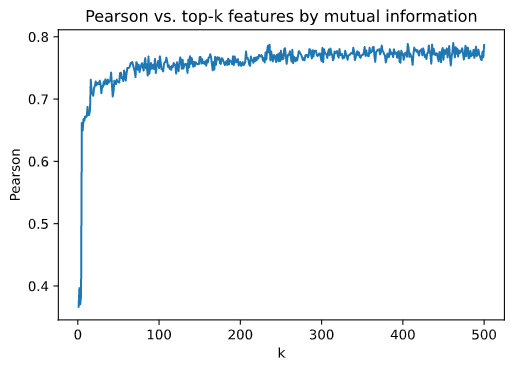
\includegraphics[scale=0.4]{mi.png}
  \caption{Performances of LR fitted on top-k features by mutual information (with 5-fold cross-validation).}
  \label{fig:mi}
\end{figure}

\textbf{Variance Inflation Factor (VIF)}: VIF is computed for each feature to measure contributed multicollinearity. Note that we omit this particular filter method for the submitted model, for the sake of optimizing Pearson correlation.

\paragraph{Wrapper Methods}

\textbf{Forward Feature Selection (FFS)}: Beginning with an empty feature set, each subsequent iteration appends a new feature to the existing feature set that offers the best Pearson correlation. We end the algorithm when the last added feature simply fails to sufficiently improve Pearson correlation.

\paragraph{Embedded Methods}

\textbf{Lasso \& Elastic Nets}: We consider these linear models during the subsequent training phase, which use L1 and L1/L2 regularization, respectively, to shrink regression coefficients of lesser important features \textit{during} fitting. Lasso \citep{Tibshirani.x} is intruiging due to its ability to reduce the high dimensionality of our feature set (relative to training set size) during fitting. Elastic Net \citep{10.2307/3647580} may succeed particularly in the presence of highly intercorrelated features.

\subsubsection{Training}

Prior to training, we standardize all features to have approximately zero mean and unit variance. For the single word subtask, we fit Linear Regression, Lasso Regression, Elastic Net Regression, Support Vector Regression (with linear kernel),  Support Vector Regression (with radial basis function kernel), K-Nearest Neighbors Regression, and XGBoost Regression models. 

After identifying the best performing model in terms of Pearson correlation, we mitigate the imbalanced nature of the target variable, ie. the multitude of class-1,2,3 samples and relative lack of class-4,5 samples. We devise a sister version of our top-performing model, fit upon a \textit{reduced} training set containing fewer class-1,2,3 samples. We tune the exact percentages removed from each class by performing cross-validation on the training set.

\subsection{System based on Feature Learning and Transfer Learning}
\begin{itemize}
  \item Reiterate the potential influence of context on lexical complexity.
  \item What MT-DNN is and its advantages, namely the ability to initialize with BERT pretrained weights.
\end{itemize}

\subsubsection{Architecture}
\begin{itemize}
  \item How BERT works and its advantages.
  \item Specify that we are using BERT cased base model, cased being preferable to uncased according to experiments.
\end{itemize}

\subsubsection{Input Layer}
\begin{itemize}
  \item For the single token subtask, how we pass sentence-target word pairs into MT-DNN model.
  \item For the multi token subtask, how we analogously pass sentence-phrase pairs into the MT-DNN model.
  \item How inputs are tokenized by BERT.
\end{itemize}

\subsubsection{Output Layer}
\begin{itemize}
  \item What the MT-DNN model produces.
  \item Explain choice to use predictions of the MT-DNN model as opposed to, say, the averaged BERT embeddings of the final layers.
  \item What is BERT attention mechanism, and how one can interpret it.
\end{itemize}

\subsection{Ensembles}
\begin{itemize}
  \item For single token subtask, how we compute a weighted average of the both feature engineering-based model predictions (ie. predictions with and predictions without data reduction) and the feature learning-based model predictions.
  \item For multi token subtask, how we harness the feature engineering-based and feature learning-based models fitted for the single token subtask, to predict two sets of predicted complexities for the head and tail words.
  \item How we then compute a weighted average of the predicted complexities of the head and tail words, and the predicted complexities of the feature engineering-based model.
  \item Note that for both subtasks, we tune weights using cross-validation upon each train set.
\end{itemize}

\section{Experiments}

\begin{itemize}
  \item Describe baseline systems.
  \item Show table of results (on trial and test sets) for all single token subtask models (for each of the feature selection techniques we tried) with MAE, Pearson, Spearman, and competition ranking.
  \item Show table of results (on trial and test sets) for all multi word-expression subtask models (for both disappointing and improved models) with MAE, Pearson, Spearman, and competition ranking.
  \item Include baseline system performances in each table.
\end{itemize}

\section{Analysis \& Discussion}

\subsection{Performance}

\begin{itemize}
  \item How we tried the said feature selection strategies through experiments on the train set, and found ensemble-based techniques regressors such as XGBoost to be the more successful algorithms, though simple linear regression performs reasonably well too.
  \item How each model performed in relation to another.
  \item How the disappointing multi word-expression model was designed, why it struggled, and what inspired our changes to it.
  \item Why latest model struggles on trial set but succeeds on cross-validation on the train set (and on the test set).
\end{itemize}

\subsection{Feature Contribution}

\begin{itemize}
  \item Show table of feature importance scores for the best performing model single token model.
  \item Discuss the most important features.
\end{itemize}

\subsection{BERT Attention}

\begin{itemize}
  \item (If we have room) Show heatmap of attention head importances (attention weights averaged across all samples).
  \item For 2-3 of most important attention heads, show the attention maps for actual samples.
  \item What (if any) patterns do the most important attention heads demonstrate.
  \item Whether these patterns surprising/expected in the context of predicting lexical complexity.
\end{itemize}

\section{Conclusion \& Future Work}
\begin{itemize}
  \item Any avenues for improvement, including synthetic data generation to improve Pearson correlation on extremely difficult samples.
\end{itemize}

\bibliographystyle{acl_natbib}
\bibliography{anthology,acl2021}

%\appendix

\end{document}
